\documentclass[10pt,a4paper]{article}

\usepackage[margin=0.62in,top=0.55in,bottom=0.62in]{geometry}
\usepackage[T1]{fontenc}
\usepackage{newtxtext,newtxmath}
\usepackage[varqu]{inconsolata}
\usepackage{amsmath}
\usepackage{booktabs}
\usepackage{tabularx}
\usepackage[expansion=false]{microtype}
\usepackage{enumitem}
\usepackage{xurl}
\usepackage[hidelinks]{hyperref}
\usepackage{xcolor}
\usepackage{tikz}
\usetikzlibrary{arrows.meta,positioning,calc}
\usepackage{pgfplots}
\pgfplotsset{compat=1.16}
\usepackage{caption}
\captionsetup{font=footnotesize,labelfont=bf,skip=2pt}
\usepackage{graphicx}

\usepackage{titlesec}
\titlespacing*{\section}{0pt}{5pt}{2pt}
\titlespacing*{\paragraph}{0pt}{2pt}{5pt}
\titleformat*{\section}{\large\bfseries\color{ink}}
\setlength{\textfloatsep}{5pt}
\setlength{\floatsep}{4pt}
\setlength{\intextsep}{4pt}
\setlist{nosep,leftmargin=1.1em}
\setlength{\parskip}{2pt}
\setlength{\parindent}{0pt}
\setlength{\tabcolsep}{4pt}
\raggedbottom
\setlength{\emergencystretch}{2em}

% ---------- colours ----------
\definecolor{ink}{HTML}{1A365D}
\definecolor{cA}{HTML}{2B6CB0}   % blue
\definecolor{cB}{HTML}{DD6B20}   % orange
\definecolor{cC}{HTML}{2F855A}   % green
\definecolor{cD}{HTML}{805AD5}   % purple
\definecolor{cG}{HTML}{718096}   % grey

\begin{document}

% ---------- Title Page ----------
\begin{titlepage}
\centering
\vspace*{1.2cm}

\IfFileExists{iitd.png}{{\includegraphics[width=4.2cm]{iitd.png}}}{}

\vspace{1.0cm}

{\huge\scshape Indian Institute of Technology Delhi\par}

\vspace{0.4cm}

{\Large COL764: Information Retrieval and Web Search\par}

\vspace{2.2cm}

{\rule{0.85\textwidth}{0.8pt}\par}
\vspace{0.6cm}
{\LARGE\bfseries Assignment 4: Iterative Retrieval for Multi-hop\\[4pt] Question Answering\par}
\vspace{0.6cm}
{\rule{0.85\textwidth}{0.8pt}\par}

\vspace{2.5cm}

{\Large\bfseries Instructor\par}
\vspace{0.25cm}
{\Large Prof.\ Srikanta Bedathur\par}

\vspace{1.2cm}

{\Large\bfseries Submitted by\par}
\vspace{0.25cm}
{\Large Aditya Anand\par}
\vspace{0.1cm}
{\large 2023CS50284\par}

\vfill

{\Large \today\par}

\vspace{1cm}

\end{titlepage}

% =====================================================================
\newpage

\section*{Overview}
Two-hop questions need a second paragraph about an entity the question does not name (the \emph{bridge}). The
agent first splits the question into Q1 and Q2, where Q2 refers to Q1's answer as \#1. It answers Q1 from retrieved
passages, searches again with the bridge and answers Q2. LLM calls left over are used to check the answer.

\begin{center}
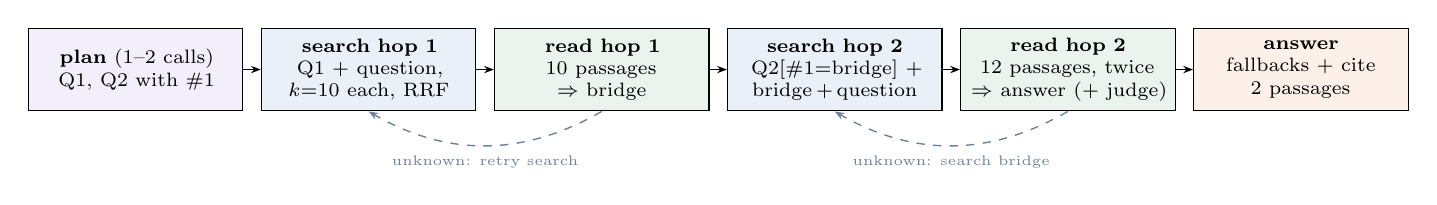
\begin{tikzpicture}[font=\scriptsize, node distance=0.22cm,
  st/.style={draw=black, line width=0.4pt, align=center, text width=2.55cm, inner sep=2.5pt, minimum height=1.05cm},
  arr/.style={-{Stealth[length=3.5pt]}, black, line width=0.5pt}]
  \node[st, fill=cD!10] (p) {\textbf{plan} (1--2 calls)\\Q1, Q2 with \#1};
  \node[st, fill=cA!10, right=of p] (s1) {\textbf{search hop 1}\\Q1 + question, $k{=}10$ each, RRF};
  \node[st, fill=cC!10, right=of s1] (r1) {\textbf{read hop 1}\\10 passages\\$\Rightarrow$ bridge};
  \node[st, fill=cA!10, right=of r1] (s2) {\textbf{search hop 2}\\Q2[\#1=bridge] + bridge\,+\,question};
  \node[st, fill=cC!10, right=of s2] (r2) {\textbf{read hop 2}\\12 passages, twice\\$\Rightarrow$ answer (+ judge)};
  \node[st, fill=cB!10, right=of r2] (a) {\textbf{answer}\\fallbacks + cite 2 passages};
  \foreach \u/\v in {p/s1,s1/r1,r1/s2,s2/r2,r2/a} \draw[arr] (\u) -- (\v);
  \draw[arr, dashed, cG] (r1.south) to[out=-150,in=-30] node[below, font=\tiny]{unknown: retry search} (s1.south);
  \draw[arr, dashed, cG] (r2.south) to[out=-150,in=-30] node[below, font=\tiny]{unknown: search bridge} (s2.south);
\end{tikzpicture}
\end{center}

% =====================================================================
\section{Single-shot vs.\ iterative}
\begin{minipage}[t]{0.585\textwidth}
\vspace{0pt}
\centering\footnotesize
\begin{tabular}{@{}lcccccc@{}}
\toprule
Dev set, 300 questions & EM & Ans.\ F1 & Ev.\ F1 & $S$ & Search & LLM\\
\midrule
B1 single-shot (starter) & 0.1400 & 0.2110 & 0.3717 & 0.2431 & 1.00 & 1.00\\
B2 staff iterative (leaderboard) & 0.2033 & 0.2596 & 0.4767 & 0.3030 & 2.03 & 3.03\\
\textbf{My agent (final)} & \textbf{0.4967} & \textbf{0.5965} & \textbf{0.6650} & \textbf{0.6102} & 4.37 & 5.25\\
\bottomrule
\end{tabular}
\captionof{table}{$S = 0.8\cdot$Ans.\ F1$\,+\,0.2\cdot$Ev.\ F1. Search, LLM: mean calls per question. All 300 questions ran without errors.}
\label{tab:main}
\end{minipage}\hfill
\begin{minipage}[t]{0.395\textwidth}
\vspace{0pt}
\centering\footnotesize
\begin{tabular}{@{}lcc@{}}
\toprule
Diagnostic & B1 & Mine\\
\midrule
both gold paragraphs retrieved & 15.3\% & 69.7\%\\
hop-2 paragraph retrieved & 23.3\% & 72.3\%\\
bridge (hop-1 answer) correct & -- & 76.3\%\\
gold paragraphs cited (of 2) & 0.74 & 1.33\\
\bottomrule
\end{tabular}
\captionof{table}{Retrieval and bridge accuracy (\texttt{dev/analyze.py}).}
\end{minipage}

% =====================================================================
\section{Design}
\textbf{Plan.} One LLM call writes Q1 and Q2. The plan is asked again, with a prompt that first names the hidden
entity, if Q2 lacks \#1, if Q1 repeats at least 90\% of the question's content words, asks \emph{when} or \emph{how
many} (the bridge is always an entity), adds a place type the question does not mention or drops every name in the
question, or if the model copies a prompt example. If both attempts fail, a possessive (\emph{X's team}) or
\emph{the Y of X} phrase is split off without the LLM. Answer F1 is 0.60 with a plan and 0.48 on the 8 questions
without one.

\textbf{\texttt{next\_query}.} Each hop sends two $k{=}10$ BM25 queries with the question words removed: Q1 and
the full question at hop~1, and Q2 with the bridge filled in plus bridge + question at hop~2. Results are merged by
reciprocal rank fusion, $\sum 1/(3+\mathrm{rank})$. After a failed read, hop~1 searches with Q1 plus the first
sentence of an LLM-written guess passage (Query2doc), and hop~2 searches with the bridge alone or, for \emph{when}
questions, with the bridge plus a Query2doc sentence.

\textbf{Reading and checking.} The LLM reads 10 passages at hop~1 and 12 at hop~2, in full (none is longer than
2,000 characters). At hop~1 the article named in the question is shown first: the bridge is right 83\% of the time
when the gold passage comes first and 67\% when it is third or lower. A bridge taken from a passage that is neither the
first nor that article (47\% right) is read again after a Query2doc search, and if hop~1 keeps failing the bridge comes from the model's memory.
The hop-2 answer gets a second read with the passages reversed and the original question. If the two answers
differ, a judge call picks one and keeps the first when unsure. With calls to spare, the model also answers Q2
without passages, and the judge decides again if a passage supports that answer. In the final run these checks
replaced 21 answers, 9 for the better and 1 for the worse.

\textbf{\texttt{should\_stop} and \texttt{answer}.} The agent stops when hop~2 has an answer of the asked type
(a date for \emph{when}, a number for \emph{how many}) that is not the bridge, or when one LLM call or 15\,s is
left. If hop~2 never answered, \texttt{answer} asks the model for a best guess with the bridge as a hint, then
falls back to a rejected hop-2 answer of the right type and then to a span from the best passage. The answer is
returned as the model wrote it. Two passages are cited: one with the bridge, preferably the article the question
names, and one with the answer, preferably also naming the bridge. If the LLM server fails a call, the agent goes
on with the budget it has left; with 5\% of calls failing, $S$ is 0.601 instead of 0.539.

\textbf{What did not help.} Asking the model to copy the answer word for word from the passage lowered $S$ by
0.049, and a third hop-2 search at the start lowered it by 0.022 because retries then had no search left. Quoting
the evidence before answering, a reasoning line, judging the bridge, 14 passages at hop~2 and Query2doc for every
question did not help either.

% =====================================================================
\section{Error analysis}
The agent gets EM $=0$ on 151 of the 300 dev questions. The automatic labels from \texttt{dev/analyze.py} are
(i)~35, (ii)~15, (iii)~42, (iv)~51 and (v)~8, against 191, 0, 15, 52 and 0 for B1. Iterating removed most bridge
failures, so reading errors are now the largest group: 209 questions reach the last read with both gold paragraphs
retrieved, and on them answer F1 is 0.74 (B1: 0.54). Many (iv) answers still get partial credit, such as
\emph{August 5, 1940} for \emph{5 August 1940} (F1 1.0, EM 0). Table~\ref{tab:err} lists 10 errors labelled by hand:
(i)~3, (ii)~2, (iii)~2, (iv)~2 and (v)~1. Only Berthelot differs from its automatic label, which is (iii) because
both gold paragraphs were retrieved.

\textbf{Example 1 (i), Johnny Berthelot.} The plan is right and the gold paragraph is ranked first. It says
Berthelot is \emph{a member of the Louisiana House of Representatives \dots\ based in his hometown of Gonzales}, so
the model returns Gonzales; the intended bridge, Baton Rouge, is only implied. Hop~2 then looks for Auburn wins at
Gonzales. The first read answers \emph{unknown}, and the guess read takes 1994 from the retrieved Auburn--LSU table,
but that game was played at Auburn; the last win at Baton Rouge was in 1999. With a wrong bridge and no hop-2
paragraph, answer F1 is 0.14 ($n{=}42$), against 0.76 ($n{=}188$) with the right bridge and the paragraph found.

\textbf{Example 2 (iii), WAJM.} The bridge (Atlantic City) and both gold paragraphs are found. Two nearly identical
census paragraphs from that article, neither dated, give household sizes of 2.50 and 2.46 (gold). The first read
answers 2.50 and the second read 2.46, and the judge keeps the first answer. No passage says which census the
question means.

\begin{center}
\footnotesize\renewcommand{\arraystretch}{1.12}
\begin{tabularx}{\textwidth}{@{}c>{\raggedright\arraybackslash}X>{\raggedright\arraybackslash}p{2.3cm}>{\raggedright\arraybackslash}p{2.6cm}>{\raggedright\arraybackslash}p{3.9cm}@{}}
\toprule
& Question (shortened) & Gold & Mine & What went wrong\\
\midrule
(i) & Last time Auburn won in the work location of Johnny Berthelot? & 1999 & 1994 & bridge \emph{Gonzales} (hometown), not \emph{Baton Rouge}\\
(i) & Sibling of the composer of \emph{Downtown}? & Astrid Young & Michael Gore & bridge \emph{Luke Laird}, writer of Lady Antebellum's \emph{Downtown}, not Neil Young\\
(i) & When did the civil war start in the country Ita Ford is from? & October 15, 1979 & April 1861 & bridge \emph{United States} (her nationality), not El Salvador\\
(ii) & Manager when Tommy Logan's team won the Champions League? & Roberto Di Matteo & Jos\'e Mourinho & bridge Chelsea right; stopped with a search left, hop-2 paragraph never retrieved\\
(ii) & When did Harrysong's country become a member of OPEC? & 1971 & the 1970s & bridge Nigeria right; vague answer accepted, OPEC table never retrieved\\
(iii) & Where did the 2007 World Series winner get Brandon Phillips from? & Los Angeles Angels & Cleveland Indians & both gold paragraphs retrieved, wrong team read\\
(iii) & Average household size in the city served by WAJM? & 2.46 & 2.50 & second read found 2.46; the judge kept 2.50\\
(iv) & When did the country of Saldus Municipality join the Soviet Union? & 5 August 1940 & August 5, 1940 & same date, other order (F1 1.0, EM 0)\\
(iv) & Forest by the southern border of Jerzy Passendorfer's death city? & Kabaty & Kabaty Forest & correct despite a wrong bridge (\emph{Skolim\'ow}); extra word (F1 0.67)\\
(v) & Who was targeted for defrauding the electoral process, in Hotel Courtland's state? & a whole sentence & John Kerry & gold answer is a sentence; hop-2 paragraph never retrieved\\
\bottomrule
\end{tabularx}
\captionof{table}{Ten errors of the final agent, labelled by hand from their traces.}
\label{tab:err}
\end{center}

% =====================================================================
\section{AI-use disclosure and code provenance}
I used Claude Code (Anthropic, Claude Opus 5.5) to read the starter code, write the agent and the analysis scripts
in \texttt{dev/}, run the experiments and draft this report. I decided what to try and what to keep, checked the
numbers, and am responsible for the submission. No external code was copied. The loop follows IRCoT (Trivedi et
al., ACL 2023) and ReAct (Yao et al., ICLR 2023), reciprocal rank fusion follows Cormack, Clarke and Buettcher
(SIGIR 2009), and the data is MuSiQue (Trivedi et al., TACL 2022). BM25, the tools and the scorer come from the
course's \texttt{a4} package. The few-shot examples were written by hand and contain no answers. The agent stores
no answers or data and never recognises a question.

\end{document}
